% ---------
% Compile with "pdflatex hw0".
% --------
% !TEX TS-program = pdflatex
% !TEX encoding = UTF-8 Unicode

\documentclass[11pt]{article}
\usepackage{jeffe,handout,graphicx}
\usepackage[utf8]{inputenc}             % Allow some non-ASCII Unicode in source
\usepackage[labelfont=bf]{caption}

% Define tabs
\newcommand\tab[1][0.5cm]{\hspace*{#1}}

% =========================================================
% Define common stuff for solution headers
% =========================================================
%%%%%%%%%%%%%%%%%%%%%%%%%%%%%%%%%%%%%%%%%%%%%%%%%%%%%%%%%%%%%%%%%%%%%%%%%%%%%%%%%%%%%%
% Project Configuration File. Used to define stuff like the project name, and so on. %
%%%%%%%%%%%%%%%%%%%%%%%%%%%%%%%%%%%%%%%%%%%%%%%%%%%%%%%%%%%%%%%%%%%%%%%%%%%%%%%%%%%%%%

\Class{CS 544--Optimization Methods in Vision and Learning}
\Semester{Fall 2017}
\Authors{2} % Change num authors is shub is joining
\AuthorOne{Akshay Mishra}{akmishr2}
\AuthorTwo{Shotaro Ikeda}{ikeda2}
% \AuthorThree{Shubhankar Agarwal}{} % Add him if he needs it

\author{
  Ikeda, Shotaro\\
  \texttt{ikeda2@illinois.edu}
  \and
  Mishra, Akshay\\
  \texttt{akmishr2@illinois.edu}
  % Add for shubshub
  % \and
  % Agarwal, Shubhankar\\
  % \texttt{mystery@illinois.edu}
}

% Project title
\def\projecttitle{L-BFGS in Reinforcement Learning}

% Define some handy macros
\newcommand{\fig}[2]{%
  % Use: \gfx{path}{opts}
  \begin{figure}[h!]
    \begin{center}
      #1
    \end{center}
    \caption{#2}
  \end{figure}
}%

% =========================================================

\usepackage{fancyhdr}

\pagestyle{fancy}
\lhead{\today}
\chead{\projecttitle{}}
\rhead{}

\title{\projecttitle{}}

\begin{document}
% ---------------------------------------------------------
\thispagestyle{empty}
\maketitle

\section{Abstract}
In current deep learning literature, first-order methods are much more common due to it's computation speed.
However, there is a similarity between \textsc{Adam} and \textsc{L-BFGS}, with computations of different version of scaling.
With this project, we show that \textsc{L-BFGS} is not an in-place replacement for \textsc{Adam} and requires a through investigation for the policy to converge.

\section{Introduction}
In class, we learned the power of second order methods and speed of convergence using those methods.
In current deep learning literature, first-order methods are much more common due to it's computation speed.
The current state of the art first order method, \textsc{Adam} computes a version of scaling using the first and second moment of the gradients, successfully becoming state-of-the-art in terms of convergence.
However, we observe the similarity between \textsc{Adam} and \textsc{L-BFGS}, since \textsc{L-BFGS} computes a different type of scaling by satisfying the secant conditions and using an approximation of the Hessian to accelerate convergence.
Knowing these two facts, we conduct an in-depth study using both optimizers on deep reinforcement learning tasks.
\subsection{Reinforcement Learning}
For our reinforcement learning algorithm, we use Q-Learning with temporal difference update.
We also use a target network, which helps stabilize learning.
For our test environment, we used OpenAI's CartPole, which is a task to balance a pole on a cart as long as possible.

\fig{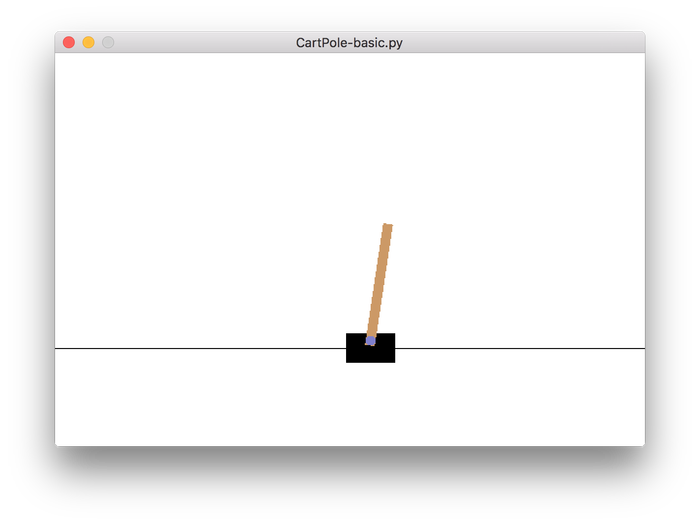
\includegraphics[width=0.3\linewidth]{assets/cartpole_ss.png}}{CartPole Environment}
\subsection{Optimizers}
We compare \textsc{Adam} and \textsc{L-BFGS}.
Here, we introduce what guided us to state the similarity between \textsc{Adam} and \textsc{L-BFGS}.
\subsubsection{\textsc{Adam} Optimizer}
The \textsc{Adam} update uses an estimate of the first and second moments of the gradients, to have either a dampening or multiplicative effect on the gradient update.

\textsc{Adam} uses the following hyper-parameters:
\begin{itemize}
\item $\beta_1$, a mixing coefficient determining the momentum of the first moment estimate
\item $\beta_2$, a mixing coefficient determining the momentum of the second moment estimate
\item $\e$, a factor to make sure division by zero does not occur.
\item $\eta$, the learning rate
\end{itemize}

These four hyper-parameters create the following rule for the $t$th update.
Suppose $\theta$ is the current set of parameters, that we wish to train. Then the update rule for $\theta$ is

\begin{align*}
  \theta \from & \theta_{t-1} \\
  g_t \from & \nabla_\theta f_\theta(x) \\
  m_t \from & \beta_1 \cdot m_{t-1} + (1 - \beta_1) \cdot g_t \\
  v_t \from & \beta_2 \cdot v_{t-1} + (1 - \beta_2) \cdot g_t^2 \\
  \hat{m_t} \from & \frac{m_t}{1 - \beta_1^t} \\
  \hat{v_t} \from & \frac{v_t}{1 - \beta_2^t} \\
  \theta_t \from & \theta_{t-1} - \eta \cdot \frac{\hat{m_t}}{\sqrt{v_t} + \e}
\end{align*}

Notice here, that the update rule is not explicitly based off of the gradient calculation $g_t$ by itself.
The \textsc{Adam} calculates estimates for the first and second moments, using those to obtain a some notion of scaling the gradient.

\subsubsection{\textsc{L-BFGS} Optimizer}
\textsc{L-BFGS} update on the other hand, uses a rough estimate of the Hessian with some constraints.

Let $\alpha$ be the step size. Typically line search is used, but pytorch's LBFGS operates on batches and uses fixed-width instead of a line search.
In particular, the update for \textsc{BFGS} is as of follows

\begin{align*}
  \theta \from & \theta_{t} \\
  p_k \from & -B_k^{-1}\nabla_\theta \\
  s_k \from & \alpha \cdot p_k \\
  x_{k+1} \from & x_k + s_k \\
  y_k \from & \nabla_\theta(x_{k+1}) - \nabla_\theta(x_{k}) \\
  B_{k+1} \from & B_k + \frac{y_{k}y_k^T}{y_k^{T}s_k} - \frac{B_{k}s_{k}s_{k}^{T}B_k}{s_{k}^{T}B_{k}s_k} \\
\end{align*}

Notice that the step is chosen with an approximation of the inverse Hessian, $B_k$.
Since the approximation of the Hessian is a guaranteed decent direction, due to the secant conditions, it can also be thought of as another version of scaling the gradient.
\textsc{L-BFGS} is another approximation on top of this, without storing the Hessian, and keeping track of the last $h$ steps.

\section{Experiments}
For each experiment, we run the operation 5 times, and show 1 standard deviation away from each run.
\subsection{Replacing \textsc{Adam}}
We attempt to replace \textsc{Adam} by finding a set of hyper-parameters that induces stable learning for \textsc{Adam}, and seeing how well replacing by \textsc{L-BFGS} does.

\plt{base.png}{%
  Since the parameters are tuned for \textsc{Adam}, it is not surprising L-BFGS does not perform worse. However, it performs much worse.
}%

To confirm the odd behavior with \textsc{L-BFGS}, we fine tune the parameters by performing a small grid search across modifying $\alpha$, the weight for prioritizing loss in the replay buffer across batches, $\eta$ for the learning rate, and $h$ for the history size.

\begin{figure}[h!]
\minipage{0.5\textwidth}
  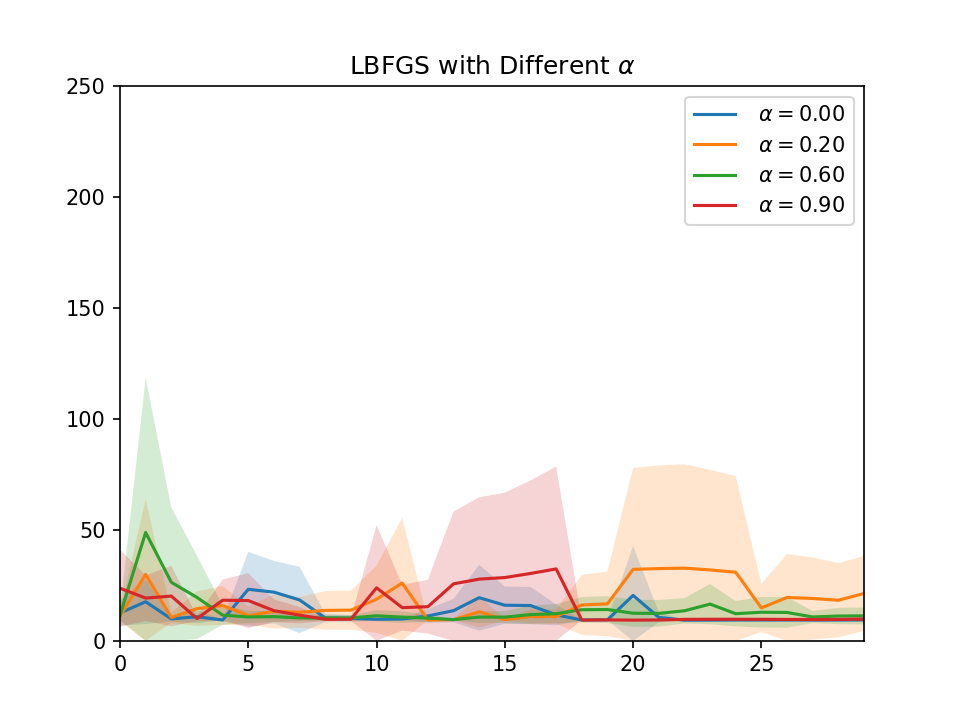
\includegraphics[width=\linewidth]{assets/lbfgs_alpha.png}
\endminipage\hfill
\minipage{0.5\textwidth}
  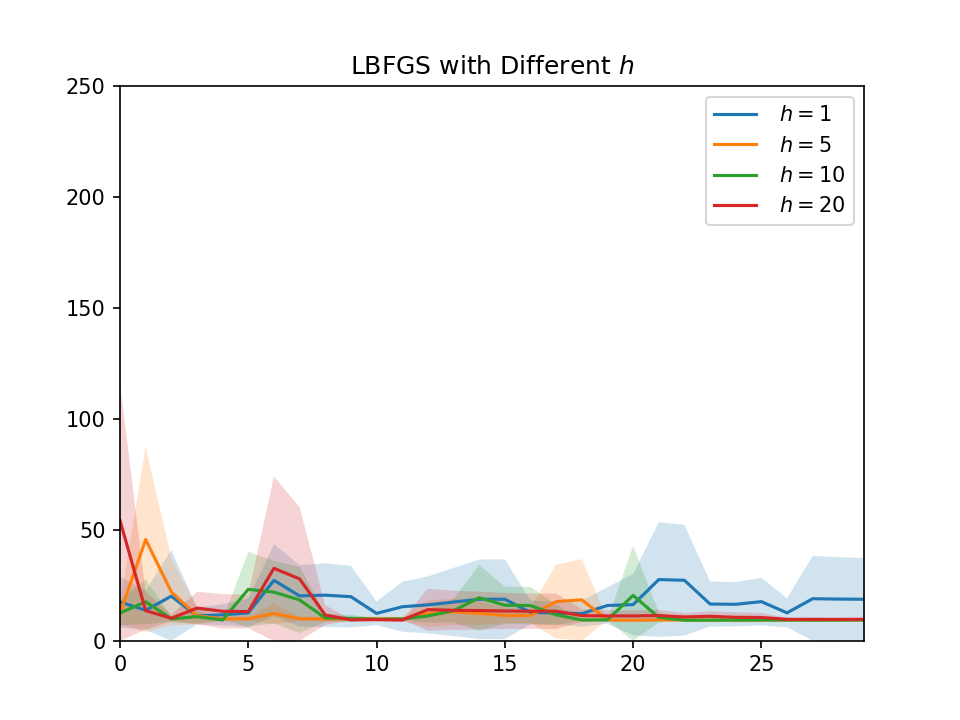
\includegraphics[width=\linewidth]{assets/lbfgs_hist.png}
\endminipage\hfill
\captionof{figure}{Various hyperparameter searches, $\alpha$ on left, $h$ on right}
\end{figure}

We found out that using LBFGS tended to explode the loss after a certain point, after which the performance of the model would not improve no matter what happened. It was not uncommon to see a loss of NaN during training.
In addition, the greater the history size, the deep net trended towards faster explosion of the loss.

\end{document}
